% 以下内容无需改动
\documentclass[UTF8,a4paper,10.5pt]{ctexart}

\usepackage{ctex}
\usepackage{geometry} %排版
\usepackage{chngcntr}
\usepackage{graphicx}%图片
\counterwithin{figure}{section}%图片按章节标号
\counterwithin{table}{section}%表格按章节标号
\usepackage{algorithm}
\usepackage{algorithmic}%算法

%\renewcommand\appendix{\setcounter{secnumdepth}{0}} 

\usepackage{url}
\usepackage[colorlinks,linkcolor=black]{hyperref} %链接

%章节数字形式
\CTEXsetup[format={\sihao\heiti}]{subsection}
\CTEXsetup[format={\wuhao\textbf}]{subsubsection}
\CTEXsetup[number={\chinese{section}}]{section}
\CTEXsetup[name={(,)}]{subsection}
\CTEXsetup[number={\chinese{subsection}}]{subsection}
\CTEXsetup[number=\arabic{subsubsection}]{subsubsection}

%页边距
\geometry{left=3cm,right=2cm,top=2.5cm,bottom=2.5cm}

%设置字号
\newcommand{\yihao}{\fontsize{26pt}{\baselineskip}}
\newcommand{\sanhao}{\fontsize{16pt}{\baselineskip}}
\newcommand{\sihao}{\fontsize{14pt}{\baselineskip}}
\newcommand{\xiaosi}{\fontsize{12pt}{\baselineskip}}
\newcommand{\wuhao}{\fontsize{10.5pt}{10.5pt}\selectfont}

%设置页眉页脚
\usepackage{fancyhdr}
\pagestyle{plain}
\lhead{}         
\chead{}           
\rhead{}           
\lfoot{}         
\cfoot{\thepage}  
\rfoot{} 



\begin{document}

%文献应用形式
\bibliographystyle{plain}

%中文题目
\begin{center}
	\sanhao{\textbf{一个简单的上海财经大学毕业论文LaTeX模板}}
\end{center}

~\\

\begin{center}
	\sanhao{\textbf{摘\quad 要}}
\end{center}

\sihao{在这里填写中文摘要。如:此文件给出一个简单的上海财经大学毕业论文LaTeX模板。其原型为上海财经大学教务处提供的\href{http://jwc.shufe.edu.cn/5126/list.htm}{Word模板}。}

\begin{flushleft}
	\sihao{\textbf{关键词:毕业论文\quad 模板\quad LaTeX}}
\end{flushleft}	

\thispagestyle{empty}
	
\pagebreak

%英文题目
\begin{center}
	\LARGE{\textbf{An Easy LaTeX Template for Sufe Thesis}}
\end{center}

~\\

\begin{center}
	\large{\textbf{Abstract}}
\end{center}

\normalsize{Write english abstract here.E.g.:This is a LaTeX template for Sufe Thesis.}.
	
\begin{flushleft}
	\normalsize{\textbf{Key words:Thesis\quad LaTeX\quad Template}}
\end{flushleft}

\thispagestyle{empty}

%目录(会自动生成)
\pagebreak
\tableofcontents

%从后面一页开始标页码
\thispagestyle{empty}
\newpage
\setcounter{page}{1}

\section{使用}

\subsection{文字}

直接打入文字即可。如:随着我国股票市场的发展完善、企业管理模式的进步、投资者理财观念的升级,证券市场上的各个主体对于能及早、准确的预测上市公司发生财务困境的需求越来越强烈。本文正是将国外非常有名的财务困境预测模型Z模型应用到我国的股票市场。由于在国内股票交易中实行的特殊政策,通常认为被实行特别处理(ST或*ST)就是公司出现财务困境的标志。因此,本文通过选取46家ST(或*ST)样本公司并对它们进行静态、动态的分析,归纳它们在被实行特别处理前五年间Z值的变化特点,找出支持这些特点的因素,从而验证了Z模型对于我国现行股市上市公司发生ST具有良好的预测能力和适用性。


\subsection{数学公式}
行内公式:逻辑回归的形式是$\ln\frac{p}{1-p}=x^T\beta$

不标号的另起一行公式:逻辑回归的形式是
$$\ln\frac{p}{1-p}=x^T\beta$$

标号的公式:逻辑回归的形式是:

\begin{equation}
	\ln\frac{p}{1-p}=x^T\beta
	\label{logistic}
\end{equation}

引用公式:公式\ref{logistic}是逻辑回归的公式。

\subsection{图片}
使用前请先确定已经在文档前方usepackage了graphicx包。随后将图片保存到和tex文件同样的路径下或者在同样的路径下建立一个figure的文件夹,随后使用相对路径引用到以下公式里即可。scale为缩放比例。

\begin{figure}[h]
	\centering
\includegraphics[scale=0.4]{sufestat.jpg}
	\caption{上海财经大学统计与管理学院院徽}
	\label{sufestat}
\end{figure}
	
\begin{figure}[h]
	\centering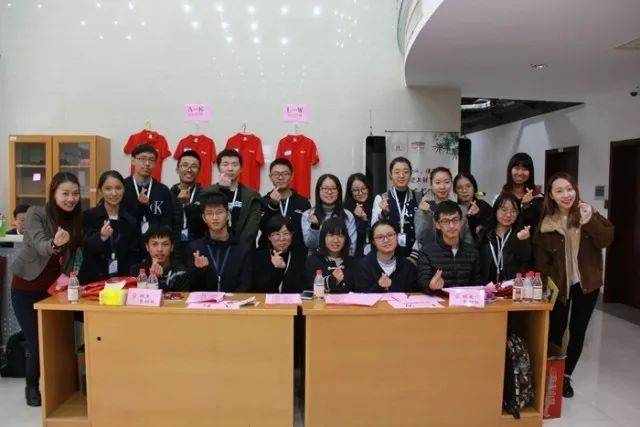
\includegraphics[scale=0.4]{sufe100.jpg}
	\caption{上海财经大学统计与管理学院100年校庆拍摄图片}
	\label{sufe100}
\end{figure}
	
图\ref{sufestat}为我院的院徽,图\ref{sufe100}中发现了许多熟悉的面孔,虽然分辨率较低。两张图均来源于百度,请不要怪我哈哈哈。至于为什么有些时候图片到下一页去了,这是一个极其基础的LaTeX问题。

\subsection{表格}
推荐一个制作LaTeX表格的\href{https://www.tablesgenerator.com/}{网站}。可以在线操作,也可以从Excel或csv文件导入,十分方便。不过该链接可能需要外网。或者下载\href{https://ctan.org/tex-archive/support/excel2latex/}{Excel2Latex}插件直接从Excel文件生成LaTeX代码。

\begin{table}[h]
	\caption{数据集}
	\centering\begin{tabular}{c|c|c}
		\hline
		序号 & 变量A & 变量B \\ 
		\hline
		1 & 2.5 & 3.4 \\ 
		\hline
		2 & 2.7 & 4.5 \\ 
		\hline
	\end{tabular}
	\label{dataset}
\end{table}

\begin{table}[h]
	\caption{回归结果}
	\centering\begin{tabular}{c|c|c|c}
		\hline
		序号 & 系数 & 标准差 & p值 \\ 
		\hline
		$\beta_0$ & 2.5 & 0.7 & <0.001 \\ 
		\hline
		$\beta_1$ & 2.7 & 0.3 & <0.001 \\ 
		\hline
	\end{tabular}
	\label{outcome}
\end{table}

表\ref{dataset}是数据集,表\ref{outcome}是回归结果。

\subsection{算法}

以自编码器算法为例:请先引入algorithm和algorithmic包。

\begin{algorithm}[H]
	\renewcommand{\algorithmicensure}{\textbf{输出:}}
	\caption{自编码器}
	\label{AutoEncoder}
	\begin{algorithmic}[1]
		\STATE 初始化:初始化编码器$\phi$和解码器$\psi$的参数
		\FOR{总回合数}
		\FOR{回合内的每个批次}
		\STATE 计算损失函数$L(\theta)=\sum_j\min||x_j-(\psi\cdot\phi)(x_j;\theta)||^2$
		\STATE 对$\theta$进行梯度下降:$\theta\gets\theta-\alpha\nabla_\theta L(\theta)$
		\ENDFOR
		\ENDFOR
		\ENSURE  编码器$\phi$和解码器$\psi$
	\end{algorithmic}  
\end{algorithm}

算法\ref{AutoEncoder}是自编码器的算法步骤。

\section{引用}
请在tex文件的同一文件下,创建一个bibfile.bib文件,在其中保存bibtex格式。在文章的最后会自动生成。在文中引用时,如下:\cite{AlexNet}和\cite{ResNet}是工程领域应用量最高的两片文章。

事实上,我觉得这样就已经足够了。但为了内容再多一点,再来几段凑一下字数。

\section{一级标题}

\subsection{二级标题}

\subsubsection{三级标题}

\subsubsection*{不标号的三级标题}

标题这样打。


\section*{附录}
\addcontentsline{toc}{section}{附录}
这里写附录。

\pagebreak
\clearpage
\phantomsection
\addcontentsline{toc}{section}{参考文献}
\bibliography{bibfile}



\pagebreak
\section*{致谢}
\addcontentsline{toc}{section}{致谢}

谢谢大家!



\end{document}